\documentclass[12pt]{article}
%\documentclass[border=0.1cm]{standalone}
\usepackage{wasysym}
\usepackage{phonenumbers}
\usepackage{marvosym }
\usepackage{xcolor}
\usepackage{comment}
\usepackage{pdfpages}
\usepackage[super]{nth}
\usepackage[paperwidth=8.5in,paperheight=11in,margin=0.5in]{geometry} 
\usepackage[UKenglish]{babel}
\usepackage[UKenglish]{isodate}% http://ctan.org/pkg/isodate
\usepackage{hyperref}
\hypersetup{
  colorlinks   = true, %Colours links instead of ugly boxes
  urlcolor     = black, %Colour for external hyperlinks
  linkcolor    = black, %Colour of internal links
  citecolor   = black %Colour of citations
}
\usepackage[final]{microtype}
\frenchspacing
\usepackage[nodayofweek,level]{datetime}
\usepackage{calc,url}
\newcounter{qz}\setcounter{qz}{0}
\newcommand{\qz}{%\
\setcounter{qz}{\value{qz}+1}
\textbf{In-class  \theqz}}

\newcounter{ol}{\setcounter{ol}{0}
\newcommand{\ol}{%\
\setcounter{ol}{\value{ol}+1}
{OL \theol}}

\newcounter{hw}\setcounter{hw}{0}
\newcommand{\hw}{%\
\setcounter{hw}{\value{hw}+1}
{IC \thehw}}

\makeatletter
\newcommand*{\rom}[1]{\expandafter\@slowromancap\romannumeral #1@}
\makeatother

\newcounter{ex}\setcounter{ex}{0}
\newcommand{\ex}{%\
\setcounter{ex}{\value{ex}+1}
\textbf{Exam \rom{\theex}}}

\usepackage[T1]{fontenc} 
\usepackage{fourier}
%\usepackage{tgschola} %to look retro
\newenvironment{mypar}[2]
  {\begin{list}{}%
    {\setlength\leftmargin{#1}
    \setlength\rightmargin{#2}}
    \item[]}
  {\end{list}}


\newcounter{wk}\setcounter{wk}{0}
\newcommand{\wk}{%\
\setcounter{wk}{\value{wk}+1}
\thewk \,\,}

\usepackage[nomessages]{fp}% http://ctan.org/pkg/fp


\usepackage{enumerate}
\usepackage{graphicx}
\usepackage{fontawesome}
\newcommand{\cvgithub}[1]{\renewcommand{\cvgithub}{#1}}
\usepackage{paralist}
\renewenvironment{description}[0]{\begin{compactdesc}}{\end{compactdesc}}

\newenvironment{alphalist}{
  \begin{enumerate}[(a)]
    \addtolength{\itemsep}{-0.5\itemsep}}
  {\end{enumerate}}
  \cleanlookdateon% Remove ordinal day reference
  \newcommand{\RomanNumeralCaps}[1]
      {\MakeUppercase{\romannumeral #1}}

\usepackage{xspace}
\makeatletter
\DeclareRobustCommand{\maybefakesc}[1]{%
  \ifnum\pdfstrcmp{\f@series}{\bfdefault}=\z@
    {\fontsize{\dimexpr0.8\dimexpr\f@size pt\relax}{0}\selectfont\uppercase{#1}}%
  \else
    \textsc{#1}%
  \fi
}
\newcommand\AM{\,\maybefakesc{am}\xspace}
\newcommand\PM{\,\maybefakesc{pm}\xspace}
\makeatother

 \newcommand{\coursename}{ Calculus II with Analytic Geometry}
\newcommand{\coursenumber}{MATH 202}
\newcommand{\sectionnumber}{01}
\newcommand{\term}{Spring }
\newcommand{\room}{Discovery Hall, room  386}
\newcommand{\meetingtime}{This class meets Monday, Wednesday, and Friday  from 
12:20\PM---1:10\PM and Tuesday and Thursday 12:30\PM---1:45\PM}
\newcommand{\officehours}{ Monday, Wednesday, and Friday 9:00\AM---11:00\AM,
    Tuesday and Thursday 9:30\AM---11:00\AM, and by appointment.}


 \newcommand{\finaldateandtime}{\printdate{14/12/\the\year} 10:30\AM---12:30 \PM}
 
 

 
 \usepackage[super]{nth}
\begin{document}
\cleanlookdateon% Remove ordinal day reference
\shortdate
\printyearoff
\large
\begin{center}
    \textbf{\coursename}  \\
    {\coursenumber---\sectionnumber} \\
     {\term \the\year} \\
\end{center}

\vskip0.25in
\normalsize


\begin{center}
\begin{description}
    \item[Instructor:] Barton Willis, PhD, Professor of Mathematics
    \item[Office:]  Discovery Hall, Room 368
    \item[Office Hours: ] \officehours
   % \item[Zoom] 616 568 5706
    \item[\phone:]  \phonenumber[country=US]{3088658868}
    \item[\Email:]  \href{mailto:willisb@unk.edu}{willisb@unk.edu}
    \item[\faGithub]   \url{https://github.com/barton-willis/calculus-two}

  \end{description}
\end{center}



\subsubsection*{Important Dates}

\begin{mypar}{0.25in}{0.25in} 
  \textbf{Exam \rom{1}} \dotfill \printdate{15/9/\the\year}  \\
  \textbf{Exam \rom{2}} \dotfill  \printdate{20/10/\the\year} \\
  \textbf{Exam \rom{3}} \dotfill \printdate{17/11/\the\year} \\
  \textbf{Exam \rom{4}} \dotfill \printdate{11/12/\the\year}  1:00 \PM -- 3:00 \PM\\
  \textbf{Final exam} \dotfill  \finaldateandtime
\end{mypar}

\subsubsection*{Grading}

Your course grade will be based on twenty-five in class assignments, four midterm exams, three online homework assignments,  and a comprehensive final exam; specifically:
\FPeval{\hwpts}{round(25*6,0)}
\begin{mypar}{0.25in}{0.25in}
    \textbf{In class work}  \emph{Twenty-five six  point assignments}  \dotfill \hwpts \/ (total) \\
    \textbf{Mid-term exams \rom{1}, \rom{2}, \rom{3}} \emph{100 points each} \dotfill 300 (total)\\
     \textbf{Mid-term exam \rom{4}}    \dotfill 50 (total)\\
     \textbf{Online homework} \emph{Three twenty point assignments}  \dotfill 60 (total) \\
    \textbf{Comprehensive Final exam} \dotfill 150 (total)
\end{mypar}
If we end the term with less than \hwpts\/ points for in class work,  your inclass work  point total will be scaled to \hwpts\/ points. There will be a five point bonus that is due the first week of the term.

\FPeval{\points}{round(\hwpts+300+50+60+150,0)}

\FPeval{\F}{round(\points*0.6-1,0)}
\FPeval{\Dm}{round(\points*0.6,0)}
\FPeval{\D}{round(\points*0.633,0)}
\FPeval{\Dp}{round(\points*0.6666667,0)}

\FPeval{\Cm}{round(\points*0.7,0)}
\FPeval{\C}{round(\points*0.733,0)}
\FPeval{\Cp}{round(\points*0.7666667,0)}

\FPeval{\Bm}{round(\points*0.8,0)}
\FPeval{\B}{round(\points*0.833,0)}
\FPeval{\Bp}{round(\points*0.8666667,0)}

\FPeval{\Am}{round(\points*0.9,0)}
\FPeval{\A}{round(\points*0.933,0)}
\FPeval{\Ap}{round(\points*0.99,0)}

The following table shows the \emph{minimum} number of points (out of \points) that
are required for each of the twelve letter grades D- through A+. For
example, a point total of \Bp\/  points will earn you a grade of B+,  and 
a point total of \Am\/ points will earn you a grade of A-. If you earn a point
total of \F\/  or less, you will a failing course grade.
 
 \vspace{0.1in}
     \begin{minipage}{5.5in}
  \centering 
\begin{mypar}{0.25in}{0.25in}
    \begin{minipage}{2.5in}
        D-  \dotfill \Dm \\
        D \dotfill \D \\
        D+ \dotfill \Dp \\
        C- \dotfill \Cm  \\
        C \dotfill \C \\
        C+ \dotfill \Cp 
        \end{minipage}
    \phantom{xxxxx}
    \begin{minipage}{2.5in}
        B- \dotfill \Bm \\
        B \dotfill  \B \\
        B+ \dotfill  \Bp\\
        A- \dotfill  \Am \\
        A \dotfill  \A \\
        A+ \dotfill  \Ap
    \end{minipage}
\end{mypar} 
\end{minipage}

\subsubsection*{Class meeting time and place}

\meetingtime in \room.

\subsubsection*{Course Resources}

Our textbook is \emph{University Calculus: Early Transcendentals}, by Joel Hass, Christopher Heil, Maurice Weir, Przemyslaw Bogacki, and George Thomas, \nth{4} edition. You \emph{must} purchase access to the online homework.

For online homework, you will need an internet connected computer. I don't recommend attempting to do your homework on a phone. For class you will need a way to take class notes--either paper for a tablet with pen input (not a keyboard). If you use paper, colored pencils or pens are nice to have.


\subsubsection*{Course Calendar}

Generally, we'll adhere to the scheduled exam dates even if we are ahead or behind with coursework.  
When we are ahead or behind, the topics on the exams will be appropriately adjusted.  


\vspace{0.1in}
\noindent \textbf{Notices:}


\begin{alphalist}
   \item Midterm exams \rom{1}--\rom{3} will be given on Friday of the week they are assigned.
   
   \item Pursuant to UNK policy for a five credit class,  Midterm exam \rom{4} will be given during final exam week.
   
    \item In class work (labelled \textbf{IC}) will generally be given on Tuesday and Thursday of the week they are assigned.  

    \item For Exam weeks, we'll have just one in class work that will 
     generally be given on Thursday.
     
    \item The final exam will be given on \finaldateandtime.
    
\end{alphalist}

\vspace{0.1in}


\begin{center}
    \small
\begin{tabular}  {|l|l|l|l|l|}
\hline
\textbf{Week}  & \textbf{Week Starting} &  \textbf{Section(s)} & \textbf{Topic(s)} & \textbf{Assessments} \\
\hline \hline 
\wk    & \printdate{21/8/\the\year} &     \S6.1 -- \S6.3   & Volumes using cross-sections, Shells, Arclength &  \hw  \\
\wk    & \printdate{28/8/\the\year}   &  \S6.4 -- \S6.5   &  Areas, Work & \hw, \hw \\
\wk    & \printdate{4/9/\the\year}&      \S6.6 --\S7.1  &  Center of mass, Logarithms   &  \hw, \hw \\
\wk    & \printdate{11/9/\the\year}&     \S7.2 -- \S7.3  & Separable DEs, Hyperbolic functions   &    \hw, \ol, \textbf{\ex} \\ \hline
\wk    & \printdate{18/9/\the\year}&     \S8.1-- \S8.2  & Integration by parts, Trigonometric integrals  &    \hw, \hw \\ 
\wk    & \printdate{25/9/\the\year}   & \S8.3 -- \S8.5   & Trigonometric substitutions, Rational functions, Tables    &  \hw,  \hw     \\ 
\wk    & \printdate{2/10/\the\year} &  \S8.6 -- \S8.7  & Numerical integration, Improper integrals &  \hw, \hw \\ 
\wk    & \printdate{9/10/\the\year}    &  \S9.1 -- \S9.3  &   Sequences, Infinite series, Integral test &  \hw,  \hw  \\
\wk    & \printdate{16/10/\the\year}     & \S9.4 -- \S9.5 &  Comparison Test, Absolute convergence  & \hw,  \ol, \ex  \\ \hline
\wk    & \printdate{23/10/\the\year}   & \S9.6&  Alternating series &  \hw, \hw \\ 
\wk    & \printdate{30/10/\the\year}      &   \S9.7 & Power series    & \hw, \hw \\ 
\wk    & \printdate{6/11/\the\year}   &   \S9.8--\S9.9 & Taylor and Maclaurian series, Convergence of Tayor series  & \hw, \hw  \\
\wk    & \printdate{13/11/\the\year}  &  \S9.10--\S10.1   & Applications of Taylor series,  Plane curves   &  \hw, \ol, \ex   \\ \hline
\wk    & \printdate{20/11/\the\year} & \S10.2 -- \S10.3   & Calculus with parametric curves,  Polar Coordinates & \hw \\
\wk    & \printdate{27/11/\the\year}    &   \S10.4--\S10.5     &  Graphing polar equations,  Areas \& lengths of polar curves   &   \hw, \hw \\
\wk    & \printdate{4/12/\the\year}   &       &   Catch up or Review    &   \\ \hline
\wk   & \printdate{11/12/\the\year}     &    &    \hfill  & \ex , \textbf{ Final Exam}  \\  \hline  
\end{tabular}
\end{center}

\subsubsection*{Grading rubric}

Generally each exam question will be worth five points. These points will be assigned according to the scheme

\begin{mypar}{0.25in}{0.25in}
  {All major steps are shown and only one correct answer}  \dotfill  5 points \\
  {Initial part of work is correct, but incomplete solution} \dotfill  3 points \\
  {Work is mostly correct, but a minor correctable error}  \dotfill 3 or 4 points \\
   {Answer (either correct or not) with no work shown}  \dotfill 0 points \\
  {Work contains a major error}  \dotfill  0 points \\
  {Work (correct or not) that answers something other than the given question} \dotfill 0 points \\
\end{mypar}
I will subtract one or more points for work that is  work is messy, hard to read, or poorly organized. Minor errors
include arithmetic errors, sign errors, and recopying errors. Major errors include using bogus identities, such as
$(1+x)^2 = 1 + x^2, \frac{a+b}{a} = 1+ b, \sqrt{x+y} = \sqrt{x} + \sqrt{y},$ and $ \frac{\mathrm{d}}{\mathrm{d} x} \left(f(x) g(x) \right)
= f^\prime(x) g^\prime(x)$.



\subsubsection*{Learning Outcomes}

On completion of this course, students will be able to
 \begin{alphalist}
    \item use definite integrals to solve problems involving volume, arc length, 
       surface area, work, and center of mass. 
    \item use integration by parts, trigonometric substitution, and partial fractions 
        to evaluate definite and indefinite integrals.
    \item apply the concepts of limits, convergence, and divergence to evaluate 
        improper integrals.
    \item determine convergence or divergence of sequences and series.
    \item use Taylor and MacLaurin series to represent functions and integrate 
        functions.
    \item use parametrizations and polar coordinates to find areas and arc lengths.
 \end{alphalist}
\subsubsection* {Class Policies}



\begin{enumerate}

\item Generally, if you are ill, injured,  incarcerated, or absent for any reason (including athletics), you must turn in 
your in class work on time. Permission to turn in work late must be made in advance, otherwise work turned in 
late will earn a score of zero.

\item During class, you may use a tablet with a pen (not a keyboard) to take class notes, but  please refrain from using other electronic devices. If your device usage distracts your classmates, I will ask you to put it away. If it's my impression that you are often not paying attention in class, I reserve the right to decline to help you with homework assignments.

\item Using unauthorized materials or communication devices while taking an exam will earn you a grade of zero on that assessment.  

\item It is essential and expected for you to attend class regularly. If you miss class, 
please ask a classmate for class notes. You may ask me for a copy 
of my class notes, but I might decline--it's unlikely my notes will be of any value 
you.

\item Examinations must be taken in class, not by Zoom.

\item If you arrive to class a bit late, please enter and take your seat. If you are
habitually late for no good reason, I will ask you to make changes to your schedule.


\item For examinations and homework, show your work.  
\emph{No credit will be given for multistep problems without the necessary work. Your solution must contain enough detail
so that I am convinced that you could correctly solve any similar problem.} Also erase or clearly mark any work you want me to ignore; otherwise,
I'll grade it.  

\item The work you turn in for a grade must be \emph{accurate, 
complete, concise, neat}, and \emph{well-organized}.  
\emph{You will not earn full credit on work that falls short of 
these expectations.}

\item Class cancellations due to weather, illness, or other unplanned circumstances may require that we make  adjustments
to the course calendar, exam dates, or due dates for course assessments.  It is your responsibility to attend class and to be aware of changes the class calendar.

\item I will \emph{decline} all requests for extra credit or for redoing an assignment or examination to earn a higher grade.

\item For examinations, you may use a teacher provided quick reference sheet, but no other reference materials. You may also use a pencil, an eraser, and a scientific calculator. For examinations, your phone and all such
devices must be turned off and \emph{out of sight.} 

\item The final examination will be \emph{comprehensive} and it will be given 
during the  time scheduled by the University. Except for \emph{extraordinary circumstances}
you must take the exam at this time.
 
\item If you have questions about how your work has been graded, make an appointment with me immediately.

\item Please regularly check Canvas  to verify that your scores have 
been recorded correctly.  If I made a mistake in recording one of
your grades, I'll correct it provided you saved your paper.

\end{enumerate}

\subsubsection*{University Policies\footnote{These polices are
copied from \url{https://catalog.unk.edu/undergraduate/academics/academic-regulations/}
and from \url{https://www.unk.edu/academic_affairs/asa_forms/course-policies-and-resources.php}.
As of 29 May \the\year, these polices are current.}} 
\paragraph*{Student Attendance Policy Statement}

Students are expected to attend all meetings of classes for which they are 
registered, including the first and last scheduled meetings and the final 
examination period. Instructors hold the right and responsibility to 
establish attendance policies for their courses. Each instructor must 
inform all classes at the beginning of each semester concerning their 
attendance policies.

Participation in official University activities, serious health concerns, 
personal emergencies, and religious observances are valid reasons for absence 
from classes. Students are responsible for informing their instructors prior 
to their absence(s) from class and for completing assignments missed during 
their absence(s). No adverse or prejudicial effects shall result to any student 
with a documented, excused absence.  

Questions may be directed to the Dean of Student Affairs office or to Student 
Health \& Counseling.


\paragraph{Academic Integrity Policy}

The maintenance of academic honesty and integrity is a vital concern 
of the University community. Any student found in violation of the 
standards of academic integrity may be subject to both academic and 
disciplinary sanctions. Academic dishonesty includes, but is not 
limited to, the following:

\begin{itemize}
    \item \textbf{Cheating} Copying or attempting to copy from an academic 
    test or examination of another student; using or attempting to 
    use unauthorized materials, information, notes, study aids or 
    other devices for an academic test, examination or exercise; 
    engaging or attempting to engage the assistance of another 
    individual in misrepresenting the academic performance of a 
    student; or communicating information in an unauthorized manner 
    to another person for an academic test, examination or exercise.
    
    \item \textbf{Fabrication and falsification} Falsifying or 
    fabricating any information or citation in any academic exercise, 
    work, speech, test or examination. Falsification is the 
    alteration of information, while fabrication is the invention 
    or counterfeiting of information.

    \item \textbf{Plagiarism}  Presenting the work of another as one's 
    own (i.e., without proper acknowledgment of the source) and 
    submitting examinations, theses, reports, speeches, drawings, 
    laboratory notes or other academic work in whole or in part as 
    one's own when such work has been prepared by another person or 
    copied from another person.

    \item \textbf{Abuse of academic materials and/or equipment} 
    Destroying, defacing, stealing, or making inaccessible library 
    or other academic resource material.

    \item \textbf{Complicity in academic dishonesty} Helping or 
    attempting to help another student to commit an act of academic 
    dishonesty.

    \item \textbf{Falsifying grade reports} Changing or destroying 
    grades, scores or markings on an examination or in an 
    instructor's records.

    \item \textbf{Misrepresentation to avoid academic work} 
    Misrepresentation by fabricating an otherwise justifiable 
    excuse such as illness, injury, accident, etc., in order 
    to avoid or delay timely submission of academic work or to 
    avoid or delay the taking of a test or examination.
    
    \item \textbf{Other Acts of Academic Dishonesty} Academic units 
    and members of the faculty may prescribe and give students prior 
    written notice of additional standards of conduct for academic 
    honesty in a particular course, and violation of any such 
    standard shall constitute a violation of the Code.

\end{itemize}
Under Section 2.9 of the Bylaws of the Board of Regents of the 
University of Nebraska, the respective colleges of the University 
have responsibility for addressing student conduct solely affecting 
the college. Just as the task of inculcating values of academic 
honesty resides with the faculty, the college faculty 
are entrusted with the discretionary authority to decide 
how incidents of academic dishonesty are to be resolved. 
For more information, please visit UNK's Procedures and 
Sanctions for Academic Integrity and the Student Code of Conduct.


\paragraph{Reporting Student Sexual Harassment, Sexual Violence or Sexual Assault}

Reporting allegations of rape, domestic violence, dating violence, sexual assault, 
sexual harassment, and stalking enables the University to promptly provide support 
to the impacted student(s), and to take appropriate action to prevent a recurrence 
of such sexual misconduct and protect the campus community. Confidentiality will 
be respected to the greatest degree possible. Any student who believes they may 
be the victim of sexual misconduct is encouraged to report to one or more of 
the following resources:

\begin{itemize}
\setlength\itemsep{-0.25em}
  \item Local Domestic Violence, Sexual Assault Advocacy Agency 
      \phonenumber[country=US]{3082372599}

  \item Campus Police (or Security) \phonenumber[country=US]{3088658911}

  \item Title IX Coordinator \phonenumber[country=US]{3088658655}
\end{itemize}
Retaliation against the student making the report, whether by students or 
University employees, will not be tolerated.

\paragraph{Students with Disabilities} It is the policy of the University of Nebraska 
at Kearney to provide flexible and individualized reasonable accommodation 
to students with documented disabilities. To receive accommodation services 
for a disability, students must be registered with the UNK Disabilities Services 
for Students (DSS) office, 175 Memorial Student Affairs Building, 
\phonenumber[country=US]{3088658214} or by email 
\href{mailto:unkdso@unk.edu}{unkdso@unk.edu}  


\paragraph{Students Who are Pregnant} It is the policy of the University of Nebraska at Kearney to provide flexible and 
individualized reasonable accommodation to students who are pregnant. To receive 
accommodation services due to pregnancy, students must contact the 
Student Health office at \phonenumber[country=US]{3088658218}. The following links provide information 
for students and faculty regarding pregnancy rights: 

\begin{itemize}
\setlength\itemsep{-0.25em}
\item \url{https://thepregnantscholar.org/title-ix-basics/} 

\item \url{https://nwlc.org/resource/faq-pregnant-and-parenting-college-graduate-students-rights/}

\end{itemize}

\paragraph{UNK Statement of Diversity \& Inclusion}

UNK stands in solidarity and unity with our students of color, our Latinx 
and international students, our LGBTQIA+ students and students from other 
marginalized groups in opposition to racism and prejudice in any form, 
wherever it may exist. It is the job of institutions of higher education, 
indeed their duty, to provide a haven for the safe and meaningful exchange of 
ideas and to support peaceful disagreement and discussion. In our classes, 
we strive to maintain a positive learning environment based upon open 
communication and mutual respect. UNK does not discriminate on the basis of 
race, color, national origin, age, religion, sex, gender, sexual orientation, 
disability or political affiliation. Respect for the diversity of our backgrounds 
and varied life experiences is essential to learning from our similarities as 
well as our differences. The following link provides resources and other 
information regarding D\&I: \url{https://www.unk.edu/about/equity-access-diversity.php}.


%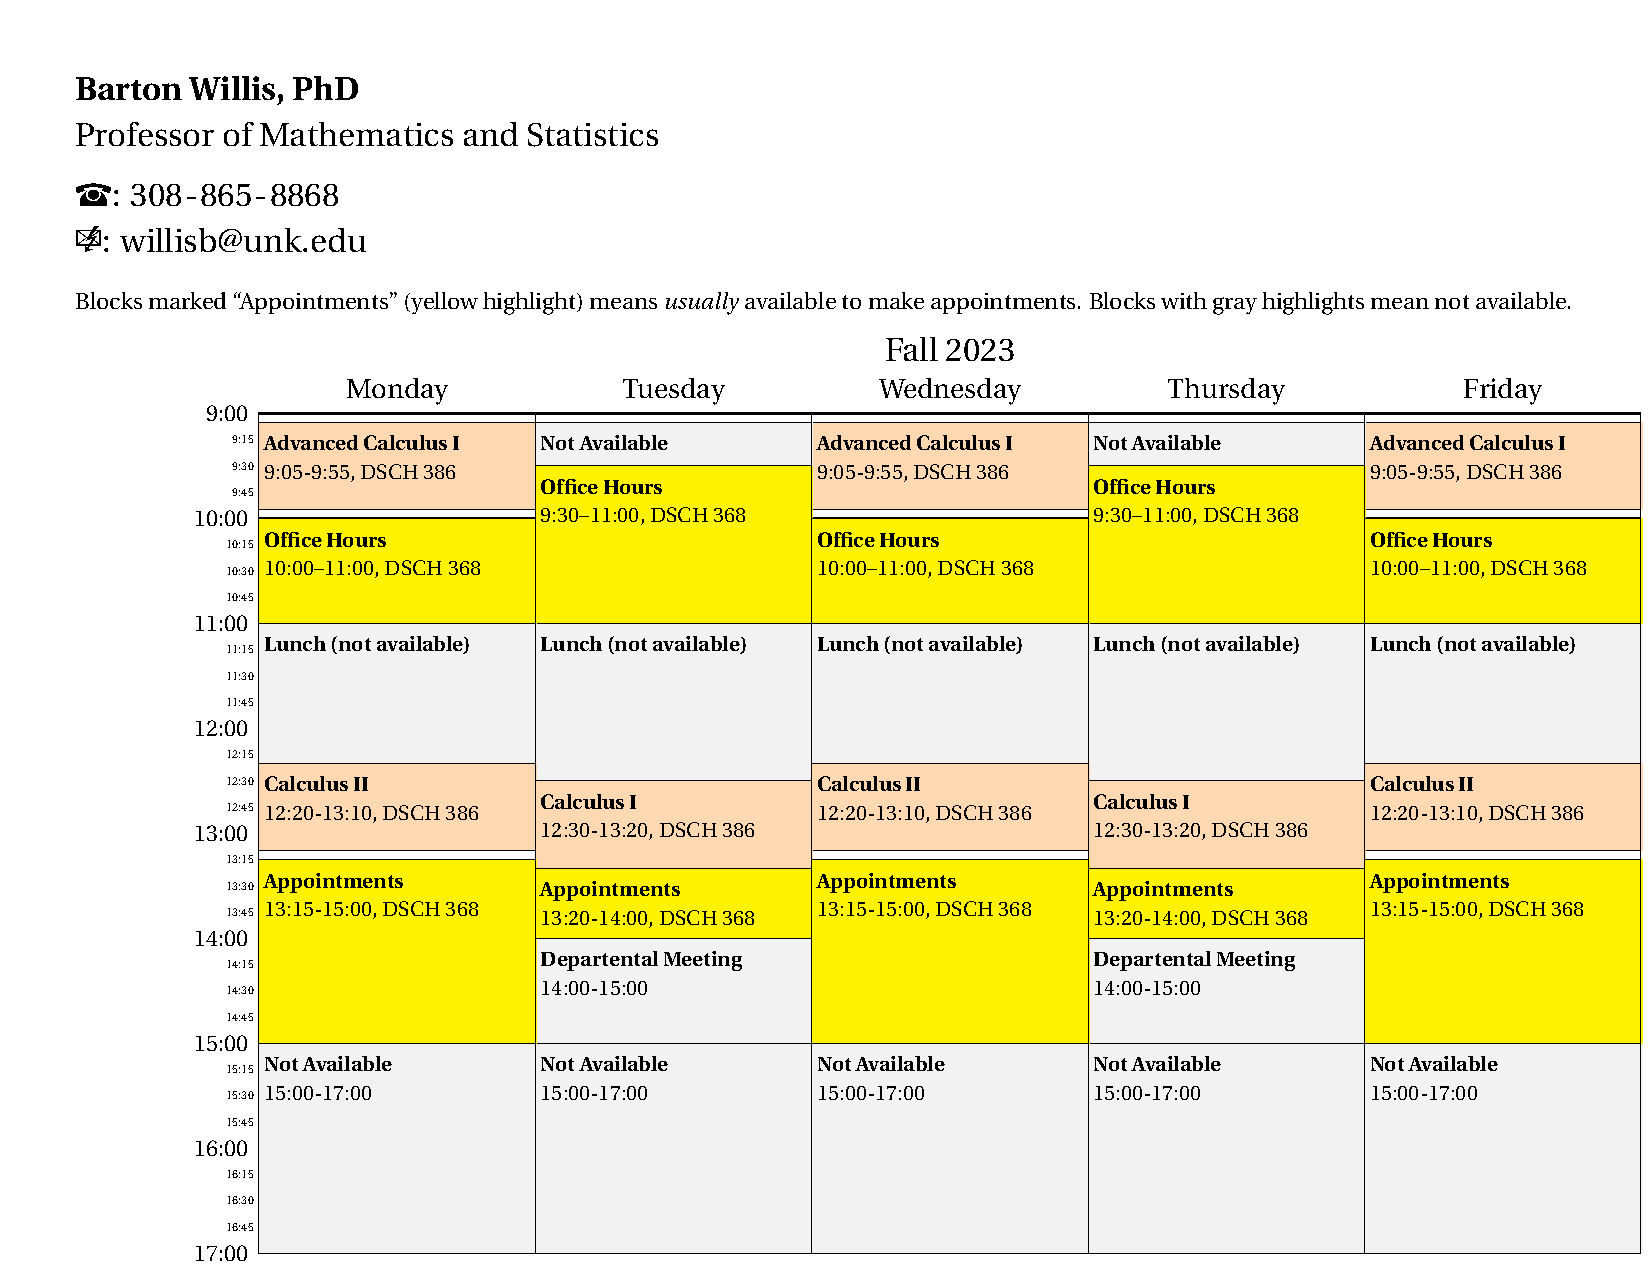
\includepdf[pages={1-},angle=90]{door_schedule.pdf}  
%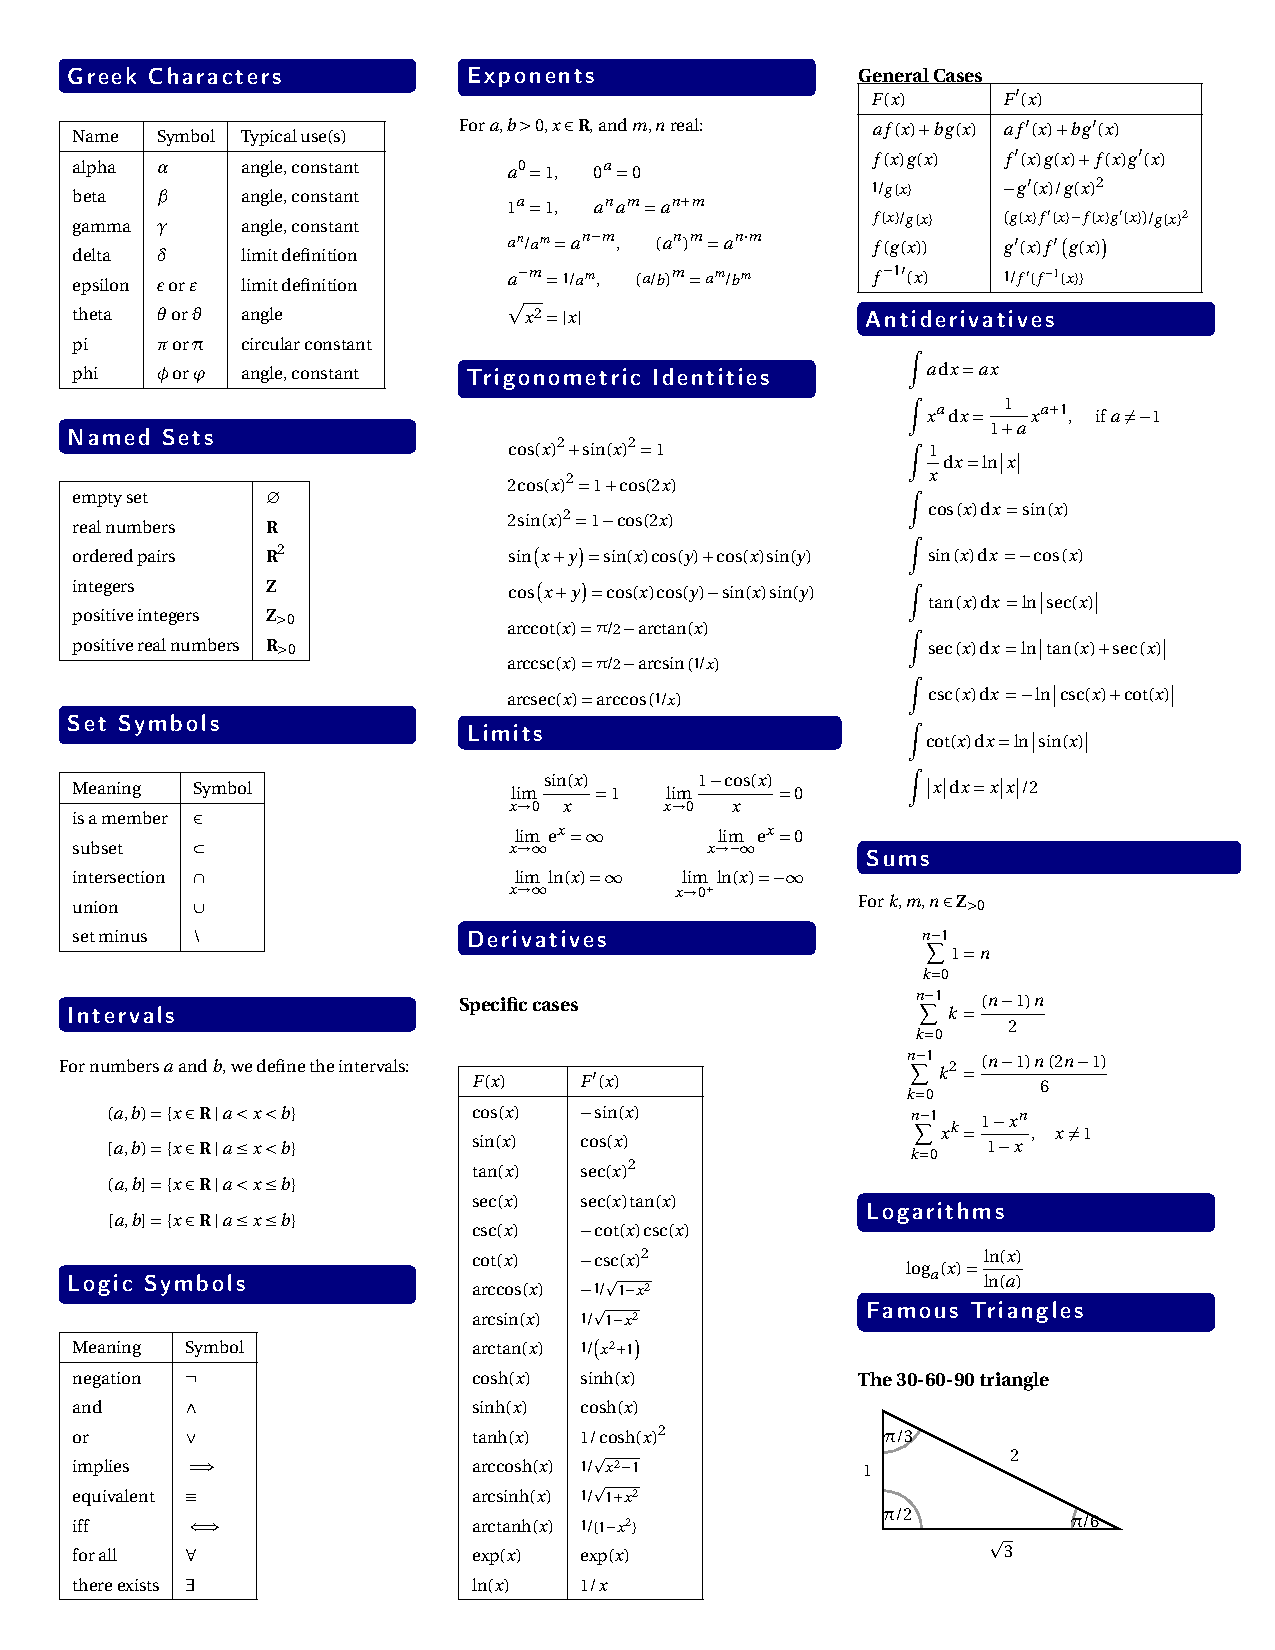
\includepdf[pages={1-},angle=90]{calculus-2-quick-reference.pdf} 
\end{document}

